%中間審査概要テンプレート ver. 3.0

\documentclass[uplatex,twocolumn,dvipdfmx]{jsarticle}
\usepackage[top=22mm,bottom=22mm,left=22mm,right=22mm]{geometry}
\setlength{\columnsep}{10mm}
\usepackage[T1]{fontenc}
\usepackage{txfonts}
\usepackage[expert,deluxe]{otf}
\usepackage[dvipdfmx,hiresbb]{graphicx}
\usepackage[dvipdfmx]{hyperref}
\usepackage{pxjahyper}
\usepackage{secdot}





%タイトルと学生番号,名前だけ編集すること
\title{\vspace{-5mm}\fontsize{14pt}{0pt}\selectfont クラウドファンディングの成功要因分析}
\author{\normalsize プロジェクトマネジメントコース 矢吹研究室 1342066 島田樹}
\date{}
\pagestyle{empty}
\begin{document}
\fontsize{10.5pt}{\baselineskip}\selectfont
\maketitle





%以下が本文
\section{背景}
クラウドファンディング\cite{wiki}を利用したプロジェクトが,SNS の発達に伴いプロジェクトの数が年々増加しており,ニュースでも報じられるようになった.クラウドファンディングとはプロジェクトの必要資金を,インターネットを利用し,不特定多数の支援者から資金提供を募集する資金調達の手法である.大手企業から個人のプロジェクトまで幅広い規模の応募が可能であり,ベンチャー企業のプロジェクトや学生の研究費用の獲得など内容は多岐にわたる.クラウドファンディングは一般的に資金提供者に対するリターンの形態よって以下の3つに分けることができる\cite{crwowd}.
\begin{enumerate}
 \item 金銭的リターンのない「寄付型」
 \item 金銭的リターンのある「投資型」
 \item 権利や物品を購入することで支援する「購入型」
\end{enumerate}

日本では金融商品取引法の規制などの関係上,購入型が最も普及しており\cite{keizai},アメリカのKickstarterをはじめ,日本のCAMPFIREやREADYFORも購入型になる.今回は日本で最初のクラウドファンディングサイトであるREADYFORとMakuakeで掲載されているプロジェクトの調達資金の時間変化を監視し成功要因を調査する.


\section{目的}
READYFORとMakuakeで掲載されているプロジェクトから,調達資金の変化をグラフ化する.動画の投稿やSNSでの告知などの多くの資金を集められた時にするべきプロジェクト実行者の行動の参考となる指標を作ることを目的とする.


\section{手法}
クラウドファンディングサイトを,毎日定時に監視し,データ収集を行う.プロジェクトの調達資金の変化をグラフ化しパターン分けをする,成功しているプロジェクトが資金を獲得している時にしている行動を考察する.


\section{想定される成果物}
プロジェクトの資金調達の情報からグラフ化しパターン分けをする.調達された日に行われた行動が成功要因であるかを判別する.

\begin{figure}[h]
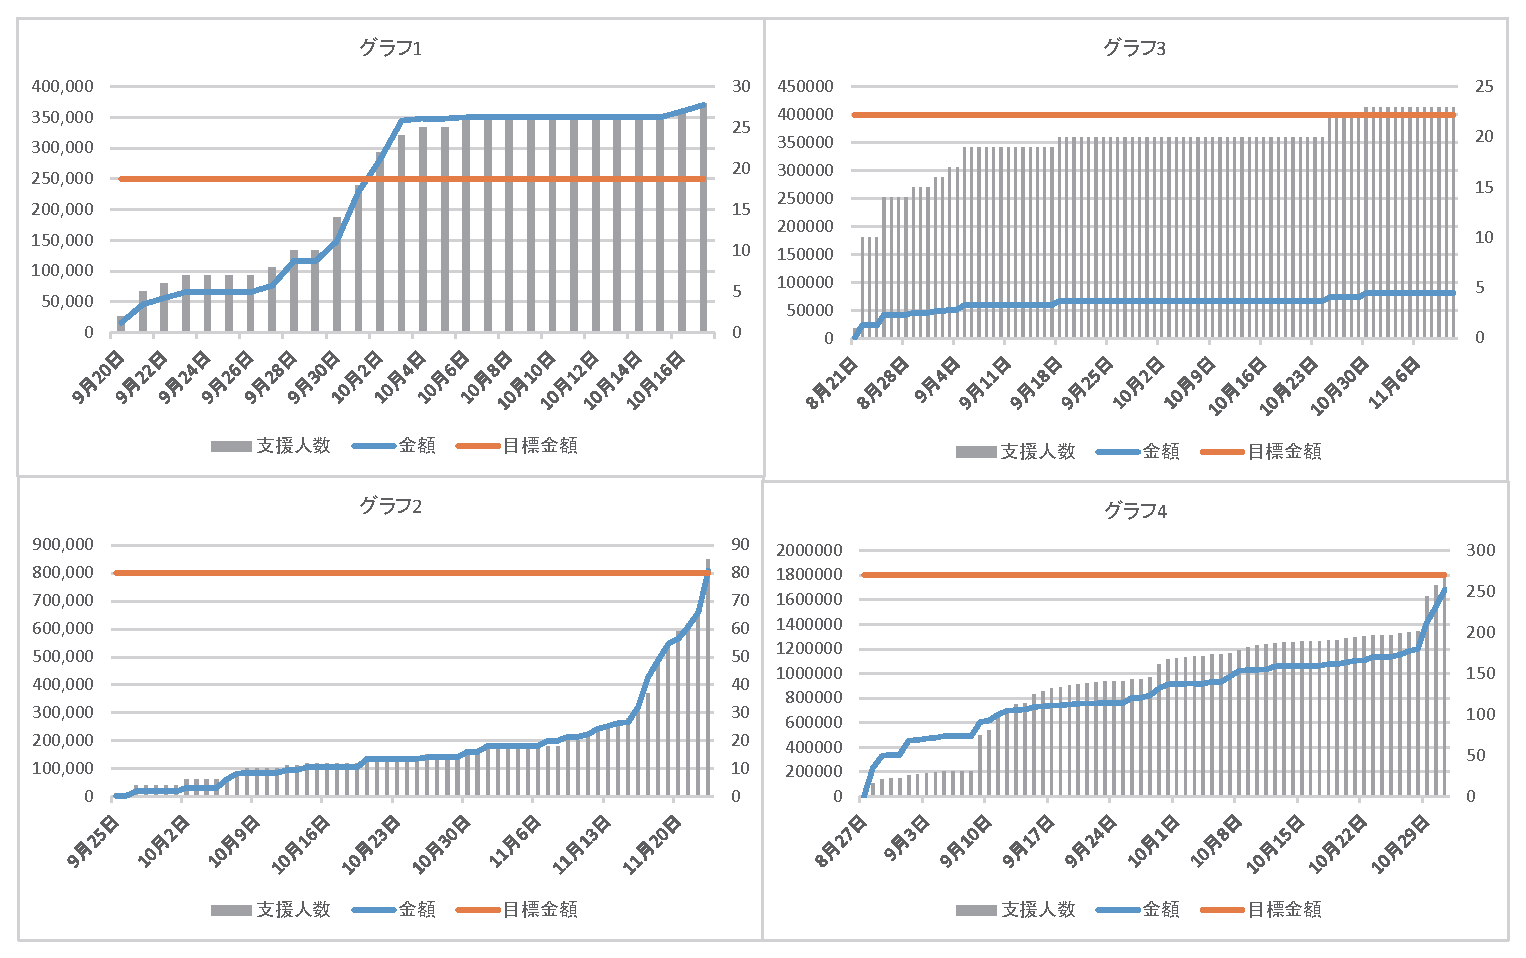
\includegraphics[width=7cm,clip]{images.pdf}
\caption{調達資金の時間変化4種類}\label{サンプル図}
\end{figure}
\section{進捗状況}
現在までに約5か月分のデータを集め,継続して収集している.集めたデータから欲しい情報だけを自動的に抜き取る方法を模索している.
\section{今後の計画}
今後は,引き続きデータを集めて資金調達の成功要因であるものの的中率を上げる.


\bibliographystyle{junsrt}
\bibliography{biblio}%「biblio.bib」というファイルが必要.

\end{document}
